\section{Introduction}

%% Background
Wide-area streaming analytics are becoming pervasive, especially with the
emerging class of Internet of Things (IoT) applications.  Large cities such as
London and Beijing have deployed millions of cameras for surveillance and
traffic control~\cite{london.surveillance, skynet}. Buildings are increasingly
equipped with a wide variety of sensors to improve energy efficiency, occupant
comfort, reliability, and
maintenance~\cite{krioukov2012building}. Geo-distributed infrastructure, such as
content delivery networks (CDNs), analyzes user requests from machine logs over the
globe~\cite{mukerjee2015practical}. These applications need to transport,
distill and process streams of data across a wide area in real time.

Although existing stream processing systems, such as
Storm~\cite{toshniwal2014storm}, Spark Streaming~\cite{zaharia2013discretized},
and VideoStorm~\cite{zhang2017live}, are capable of handling large streams of
data, they are designed to work within a single cluster, where the network is
not the bottleneck.  In contrast, the wide area network (WAN) has limited
bandwidth~\cite{hsieh17gaia, vulimiri2015global}. Recent studies show that WAN
bandwidth growth has been decelerating for many
years~\cite{global2016telegeography} while traffic demands have been growing at a staggering
rate~\cite{index2013zettabyte}.

Limited WAN bandwidth makes it neither practical nor efficient to back-haul all data to a central location.
Recent research on WAN-aware systems promotes pushing computations towards the
edge~\cite{satyanarayanan2009case, rabkin2014aggregation, pu2015low}. However,
communication is not entirely avoidable for the following reasons: $(i)$ some
analytical jobs require joining or aggregating data from multiple geo-distributed
sites~\cite{pu2015low, viswanathan2016clarinet}; $(ii)$ the edge benefits
substantially from central computing resources such as GPUs and
TPUs~\cite{abadi2016tensorflow} in the cloud; and $(iii)$
end-devices such as cameras and mobile devices suffer from limited
bandwidth in last-hop wireless links even when running processing on
nearby edge infrastructure~\cite{zhang2015design, abari2017enabling}.

% could improve efficiency (such as GDA pushes queries out; cloudlet
% etc). However, we still need data transmission for cloud off-loading or
% aggregation purpose.

When facing insufficient bandwidth, application developers need to make a
decision within the design space of data fidelity versus freshness (\autoref{fig:intro}).

\begin{figure}
  \centering
  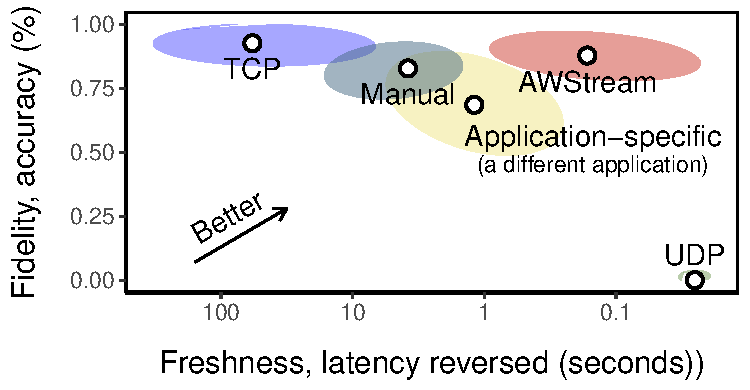
\includegraphics[width=0.9\columnwidth]{figures/figure1a.pdf}
  \caption{The trade-off space between data freshness and data fidelity when
    facing insufficient bandwidth. \autoref{sec:runtime-adaptation} describes
    the details on experiments and data for this figure.}
  \label{fig:intro}
  \vspace{-1em}
\end{figure}

Applications over existing protocols without adaptation result
extreme design points. Streaming over TCP ensures a reliable
delivery but backlogged data increases application latency. On the other hand, streaming over
UDP minimizes latency by sending packets as fast as possible, but
uncontrolled loss devastates application accuracy.

Manual policies, such as sampling, allow developers to trade data
fidelity for freshness~\cite{rabkin2014aggregation}.
However, it's difficult to write accurate policies without extensive expertise or without considerable effort.
In practice, developers write manual policies based on some set of heuristics rather than quantitative measurements.
These inaccurate policies lead to sub-optimal performance for both freshness and fidelity.

Futhermore, application-specific optimizations do not generalize. A fine-tuned
algorithm for one application will work poorly for another application, if
performance metrics or data distributions change.
For example, video streaming focuses on quality of
experience (QoE)~\cite{yin2015control}.
Because humans favor smoothness over image quality, video streaming optimizations maintain a high frame rate, e.g., 25 FPS\@.
This restriction is unnecessary for other applications, such as machine-based video analytics that maximize accuracy.

We present \sysname{}, a stream processing system that
simultaneously achieves low latency and high accuracy with minimal developer
effort. The key idea is to build an accurate and precise performance model,
instead of relying on manual or application-specific policies. \sysname{}'s
solution is three-fold: easy-to-use APIs, an automatic profiler and a
low-latency runtime.

\sysname{} augments existing stream processing operators with a new \maybe{}
operator. Its basic form takes a list of values as a knob and a function that
degrades the input stream. The knob specifies the degradation level that affects
data size and data fidelity. We extend the basic form with a library of
specialized operators for common data types, such as \texttt{maybe\_downsample}
for images. Our APIs are simple, modular and extensible. Developers do not need
to be an expert in the application domain as the knobs tolerate approximate
specifications. Multiple operators form a configuration that affects the
adaptation jointly. Arbitrary functions and external libraries can be embedded
with our operators.

\sysname{} then uses a data-driven approach to automatically build application
performance profiles with minimal developer effort. The profiles accurately
capture the relationship between application accuracy and bandwidth consumption
under different combinations of data degradation operations. We use an offline
process to bootstrap our system with developer-supplied training data, and
continuously refine the profiles online to handle potential model drifts. We
exploit parallelism and sampling-based profiling to efficiently explore the
configuration space and learn a Pareto-optimal adaptation strategy.

At runtime, \sysname{} achieves low latency by matching data rate to available
bandwidth, and high accuracy by using Pareto-optimal configurations from the
profile. Upon network congestion, our rate adaptation algorithm increases the
degradation level to reduce bandwidth demand, such that no persistent queue
builds up. To recover, it progressively decreases the degradation level after
probing for more available bandwidth. The runtime also provides additional
options for developers to control application behaviors, e.g., by limiting the
maximum allowed WAN bandwidth. For multiple applications, the
profiles allow bandwidth allocation among competing tasks for utility-fairness,
i.e.\,maximizing the minimal accuracy.

To evaluate \sysname{}, we have built three streaming applications: pedestrian
detection (PD), augmented reality (AR), and monitoring log analysis (LA). We use
real-world data to profile these applications and evaluate their runtime
performance on a geo-distributed public cloud. Our contributions and
evaluation results are as follows.

\begin{itemize}[leftmargin=16pt]

\item We propose a set of \maybe{} operators to incorporate adaptation with
  an existing stream processing model. Our programming abstraction is simple,
  modular and extensible.

\item We show that \sysname{}'s data-driven approach generates an accurate and
  precise profile for each application. Parallelism and sampling-based profiling
  can speed up the profiling substantially, up to 29X and 8X\@.

\item Using runtime experiments on geo-distributed EC2 nodes, \sysname{}
  achieves low latency and high accuracy simultaneously for all applications---sub-second latency and 5\% accuracy drop for video analytics, 4-second latency
  and 6\% accuracy drop for LA\@.

\end{itemize}

%%% Local Variables:
%%% mode: latex
%%% TeX-master: "sosp17"
%%% End:

%% LocalWords: VideoStorm, analytics, CDN, IoT
